\documentclass{MScthesisITEM}

% this package is just to generate text for demo-purposes
\usepackage{blindtext}
\usepackage{csquotes}
\usepackage{graphicx}
\usepackage{pbox}
\usepackage{float}
\usepackage{tabularx}


\title{Will a free model that is successfully proven by start-ups like Skype, Waze and \newlinetitle Snapchat work in a B2B\&C market? } % The title of your assignement; NB use \newlinetitle to start a newline
\author{Kristian Tagesen} % Your firstname and lastname
\professor{Jan Arild Audestad, ITEM} % Affiliation = ITEM for instance
\supervisor{Thomas Jelle, ITEM}

%% Uncomment the following in case you want subfigures; note that there will be a warning for the caption package
% \let\subcaption\undefined
% \let\subfloat\undefined
% \usepackage[bf]{caption}
% \usepackage{subcaption}

\DeclareGraphicsExtensions{.pdf,.jpg}
\graphicspath{{./figs/}}

\loadglsentries{glossary}
\makeglossaries

\begin{document}
\selectlanguage{english}
\pagenumbering{roman}
\pagestyle{plain}
\renewcommand{\arraystretch}{1.5}
%% Only for the project; comment out the line below for the master's thesis; the front page will be generated automatically by DAIM
\titleITEM

%% Only for the master's thesis; for the project report the description is taken from It's Learning and added by the department
\selectlanguage{english} % Change to 'norsk' if you are writing in Norwegian
\begin{titlingpage}

\noindent
\begin{tabular}{@{}p{2cm}l}
\textbf{Title:} 	& \thetitle \\
\textbf{Student:}	& \theauthor \\
\end{tabular}

\vspace{4ex}
\noindent\textbf{Problem description:}
\vspace{2ex}


MazeMap has developed an indoor map and navigation service and in less than 2 years we have helped close to 1 million users find their way. Now we want to help the next Billion. MazeMap has a very scalable technical platform and the main bottle neck achieving our goal is customer acquisition. 

To accelerate customer acquisition we are considering giving away MazeMap map service for free to customers. The free model has worked for numerous start-ups in the consumer market, e.g Skype, Waze and Snapchat, but will it work in a B2B\&C model?

Will a free model accelerate customer acquisition, in other words will e.g Universities want to help their students using MazeMap if they got the service for free or is there other factors more important than price? 

The task is to investigate if a free model will accelerate customer acquisition and if so, how should it be done?
\vspace{6ex}

\noindent
\begin{tabular}{@{}p{4cm}l}
\textbf{Responsible professor:} 	& \theprofessor \\
\textbf{Supervisor:}			& \thesupervisor \\
\end{tabular}

\end{titlingpage}
%\cleardoublepage

%% There must be an abstract in English, even though the main text is in Norwegian
\selectlanguage{english}
\pagestyle{empty}
\begin{abstract}
asdas~\cite{Author:year:XYZ}. asdad.
\end{abstract}
%\cleardoublepage

%% Only for the master's thesis; if the main text is in English and you can write Norwegian, there must be an abstract in Norwegian as well.
% \selectlanguage{norsk}
% \pagestyle{empty}
\renewcommand{\abstractname}{Sammendrag}
\begin{abstract}
\noindent Sikkerheten til nesten all offentlig nøkkel-kryptografi er basert på et vanskelig beregnbarhetsproblem. Mest velkjent er problemene med å faktorisere heltall i sine primtallsfaktorer, og å beregne diskrete logaritmer i endelige sykliske grupper. I de to siste tiårene, har det imidlertid dukket opp en rekke andre offentlig nøkkel-systemer, som baserer sin sikkerhet på helt andre type problemer. Et lovende forslag, er å basere sikkerheten på vanskeligheten av å løse store likningsett av flervariable polynomlikninger. En stor utfordring ved å designe slike offentlig nøkkel-systemer, er å integrere en effektiv ``falluke'' (trapdoor) inn i likningssettet. En ny tilnærming til dette problemet ble nylig foreslått av Gligoroski m.f., hvor de benytter konseptet om kvasigruppe-strengtransformasjoner (quasigroup string transformations). I denne masteroppgaven beskriver vi en metodikk for å identifisere sterke og svake nøkler i det nylig foreslåtte multivariable offentlig nøkkel-signatursystemet MQQ-SIG, som er basert på denne idéen.

Vi har gjennomført et stort antall eksperimenter, basert på Gröbner basis angrep, for å klassifisere de ulike parametrene som bestemmer nøklene i MQQ-SIG. Våre funn viser at det er store forskjeller i viktigheten av disse parametrene. Metodikken består i en klassifisering av de forskjellige parametrene i systemet, i tillegg til en innføring av konkrete kriterier for hvilke nøkler som bør velges. Videre, har vi identifisert et unødvendig krav i den originale spesifikasjonen, som krevde at kvasigruppene måtte oppfylle et bestemt kriterie. Ved å fjerne denne betingelsen, kan nøkkel-genererings-algoritmen potensielt øke ytelsen med en stor faktor. Basert på alt dette, foreslår vi en ny og forbedret nøkkel-genereringsalgoritme for MQQ-SIG, som vil generere sterkere nøkler og være mer effektiv enn den originale nøkkel-genereringsalgoritmen.  
\end{abstract}
% \cleardoublepage

\selectlanguage{english}% Change to 'norsk' if you are writing in Norwegian

\renewcommand{\abstractname}{Preface}
\begin{abstract}
\noindent This report consists of the preliminary work leading up to the thesis of Master of Science degree in Communication Technology at the Norwegian University of Science and Technology (NTNU). I have specialised in ICT economics at the Department of Telematics (ITEM), belonging to the Faculty of Information Technology, Mathematics and Electrical Engineering (IME).
\newline
\\
I would like to extend gratitude towards my supervisor Thomas Jelle and responsible professor Jan A. Audestad for highly valued input throughout the semester. Lastly, I wish to thank all respondents of the survey, without these answers this report would have been moot.
\end{abstract}
\cleardoublepage

% similarly you may add a separate acknowledgments page

\tableofcontents*
%\cleardoublepage

%% include if relevant
\listoffigures
%\cleardoublepage

%% include if relevant
\listoftables
%\cleardoublepage

%% include if relevant
%\listofalgorithms
%\addcontentsline{toc}{chapter}{List of Algorithms}
%\cleardoublepage

%% include if relevant
%\printglossary[title=List of Symbols, style=long]
%\cleardoublepage
\glsaddall[]

%% include if relevant
\printglossary[title=List of Acronyms,type=\acronymtype] % prints just the list of acronyms
%\cleardoublepage

\pagenumbering{arabic}
\pagestyle{ruled}
\chapter{Chapter 1 - }
%% add more chapters here
%% include here the other chapters
\chapter{Chapter 2 - Introduction}



\chapter{Chapter 3 - Methodology}

\chapter{Chapter 4 - Case Study of }

\chapter{Chapter 5 - Case Study of }



\chapter{Chapter 6 - Proposal of Business Model}




%\renewcommand*{\bibname}{References}
\bibliographystyle{unsrt}
\bibliography{references}\label{sec:references}

%% Uncomment the following if you have any appendix
\appendix
\addtocontents{toc}{%
\protect\vspace{1em}% 
\protect\noindent \bfseries \appendixtocname\protect\par
\protect\vspace{-.5em}%
}
\renewcommand{\chaptername}{\appendixname}
%% include below possible appendices (chapters)
\chapter{Invitation for the research survey}

\begin{figure}[H]
\centering

\includegraphics[width=15cm]{figs/snapshot46.png}
\caption{Invitation letter}
\label{fig:invitation_letter}
\end{figure}

\chapter{Research survey response form}
\begin{figure}
\centering
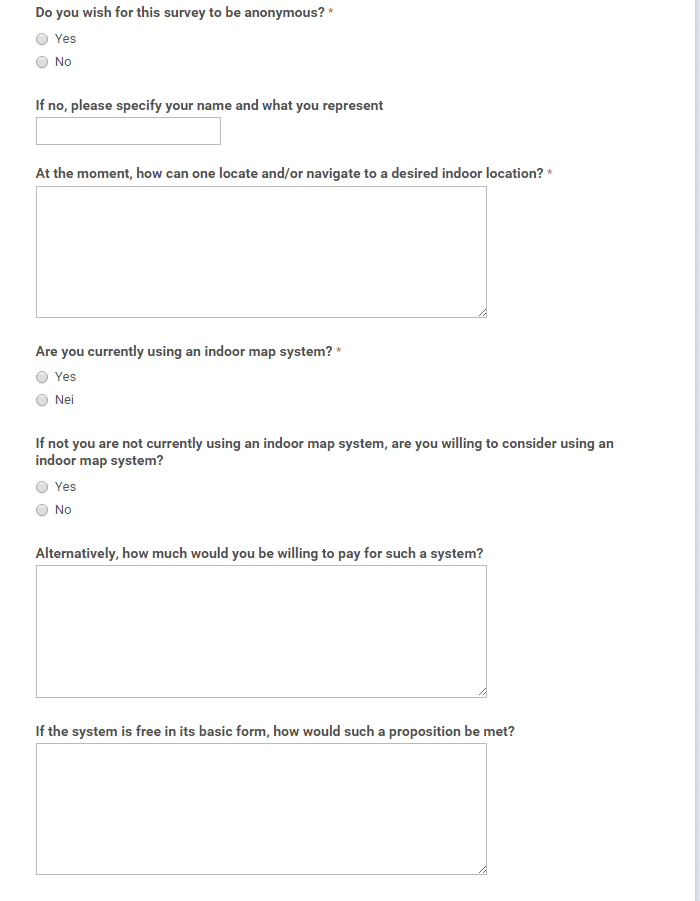
\includegraphics[width=\linewidth]{figs/questionaire1.PNG}
\caption{Screenshot of the freemium model survey response form, part 1}
\label{fig:surveyform1}
\end{figure}

\begin{figure}
\centering
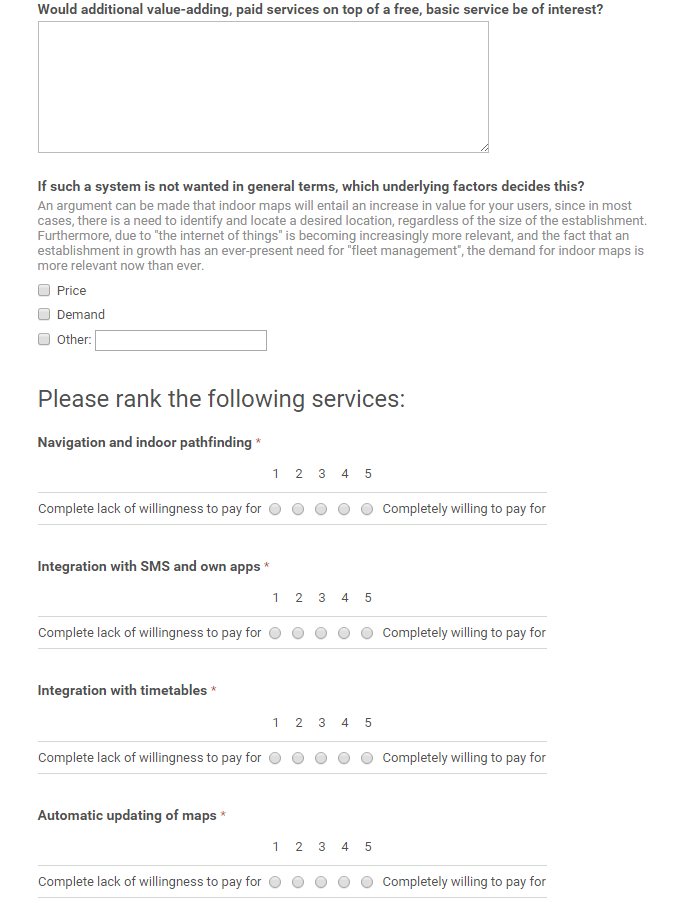
\includegraphics[width=\linewidth]{figs/questionaire2.PNG}
\caption{Screenshot of the freemium model survey response form, part 2}
\label{fig:surveyform2}
\end{figure}

\begin{figure}
\centering
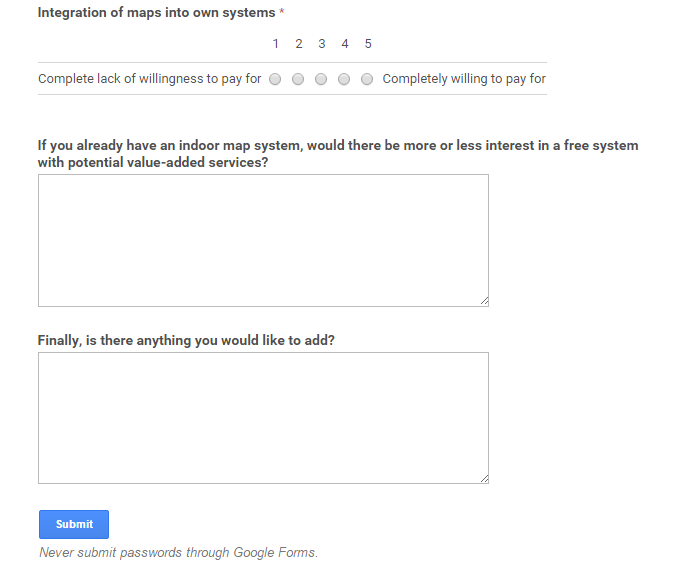
\includegraphics[width=\linewidth]{figs/questionaire3.PNG}
\caption{Screenshot of the freemium model survey response form, part 3}
\label{fig:surveyform3}
\end{figure}

\end{document} 
